\todo{graf x - coverage, y - pamat, rozne farebne krivky - pre rozne error rates.
coverage 2 5 10 20 50
error rate 0 0.1 0.2 0.5 1 2} \\
\todo{porovnanie s gkarrayom - zoberiem nejaku sadu a variujem coverage (abo error rate)} \\
\todo{graf realne data, variujem coverage (samplovanim nasimulujem ine converages)}

\begin{figure}[h]
    \centering
    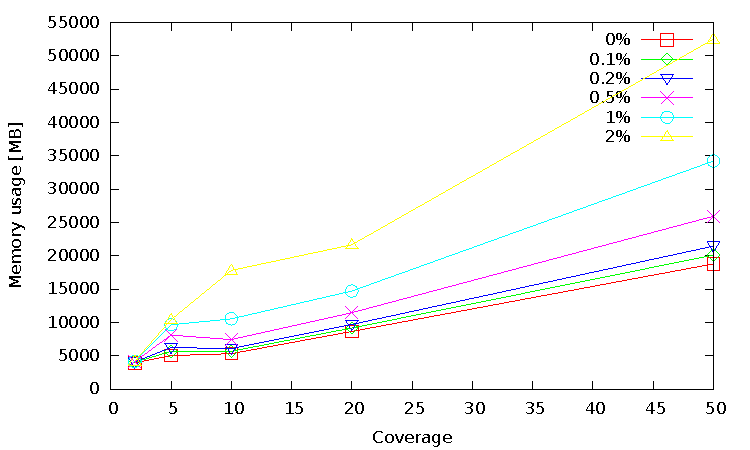
\includegraphics[width=16cm]{staphyl}
    \caption{blabla}
    \label{fig:graf_staphyl}
\end{figure}